%%%%%%%%%%%%%%%%%%%%%%%%%%%%%%%%%%%%%%%%%%%%%%%%%%%%%%%%%%%%%%%%%%%%%%%%%%%%%%%%%%
%%													
%%
%% File name: 		20hannes.tex									
%%
%% Project name:	Hochleistungsantenne								
%%
%% Type of work:	T3X00 project work								
%%
%% Author:			Sarah Brückner, Maximilian Stiefel, Hannes Bohnengel		%%
%% Date:			30th May 2016								
%%
%% University:		DHBW Ravensburg Campus Friedrichshafen						
%%
%% Comments:		Created in gedit with tab width = 4						
%%
%%													
%%
%%%%%%%%%%%%%%%%%%%%%%%%%%%%%%%%%%%%%%%%%%%%%%%%%%%%%%%%%%%%%%%%%%%%%%%%%%%%%%%%%%

\clearpage
\section{Aufbau der Bodenstation}

In diesem Abschnitt werden die von der Bodenstation der \ac{DHBW} Ravensburg zur Verfügung stehende Komponenten vorgestellt.
\subsection{Antennen}
Die Sendeleistung der Satelliten liegt typischerweise unter 1 Watt. Im 2-m-Band wäre es möglich mit einer Rundstrahlantenne ein Signal zu empfangen, 
doch auf den höheren Bändern wird aufgrund der kürzeren Wellenlänge und damit einhergehende höheren Streckendämpfung eine Richtantenne benötigt. 
Da für die Kommunikation über Satelliten beide Polarisationsarten, vertikal und horizontal, benötigt werden, kommen Kreuzyagi-Antennen zum Einsatz.  
In der unteren Grafik ist von links nach rechts eine Kreuzyagi-Antenne für das 70-cm-Band, eine Kreuzyagi-Antenne für das 2-m-Band und zwei 
Yagiantennen, welche von 90$^\circ$ um eine $\frac{\lambda}{4}$ Wellenlänge auf dem Tragrohr versetzt sind, für das 23-cm-Band, zu sehen. 
\begin{figure}[h]
	\centering
	\begin{minipage}[t]{0.3\textwidth}
		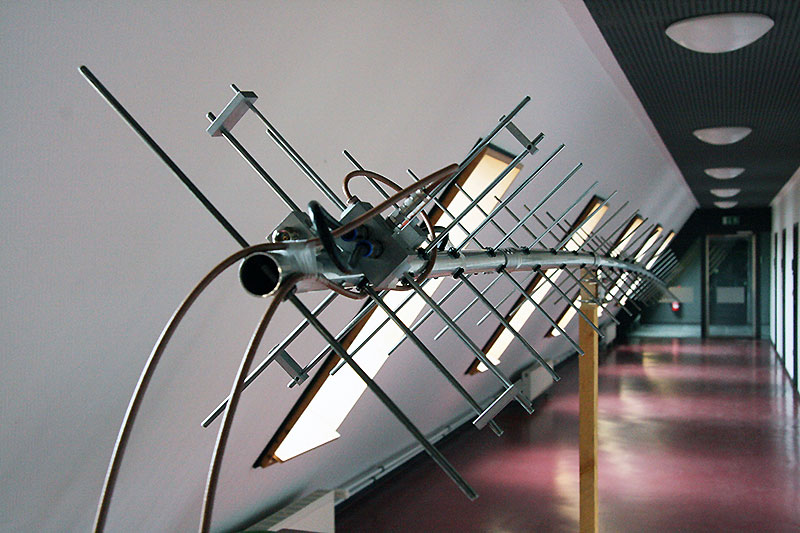
\includegraphics[width=\textwidth]{images/antenne}
	\end{minipage}
	\begin{minipage}[t]{0.34\textwidth}
		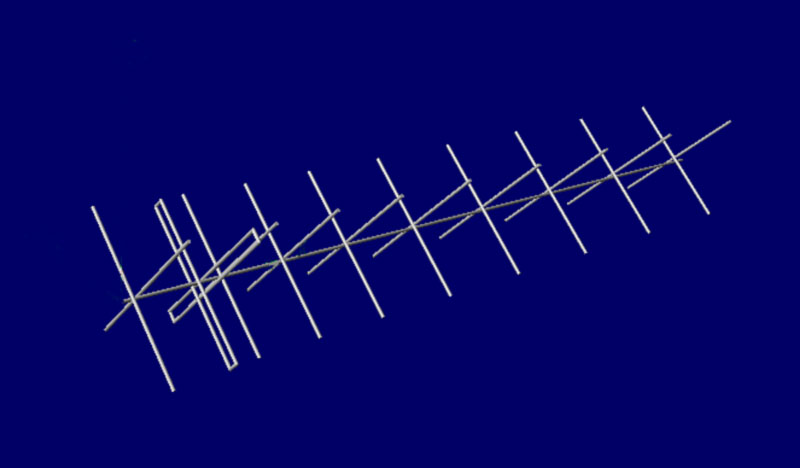
\includegraphics[width=\textwidth]{images/antenne2}
	\end{minipage}
	\begin{minipage}[t]{0.2\textwidth}
		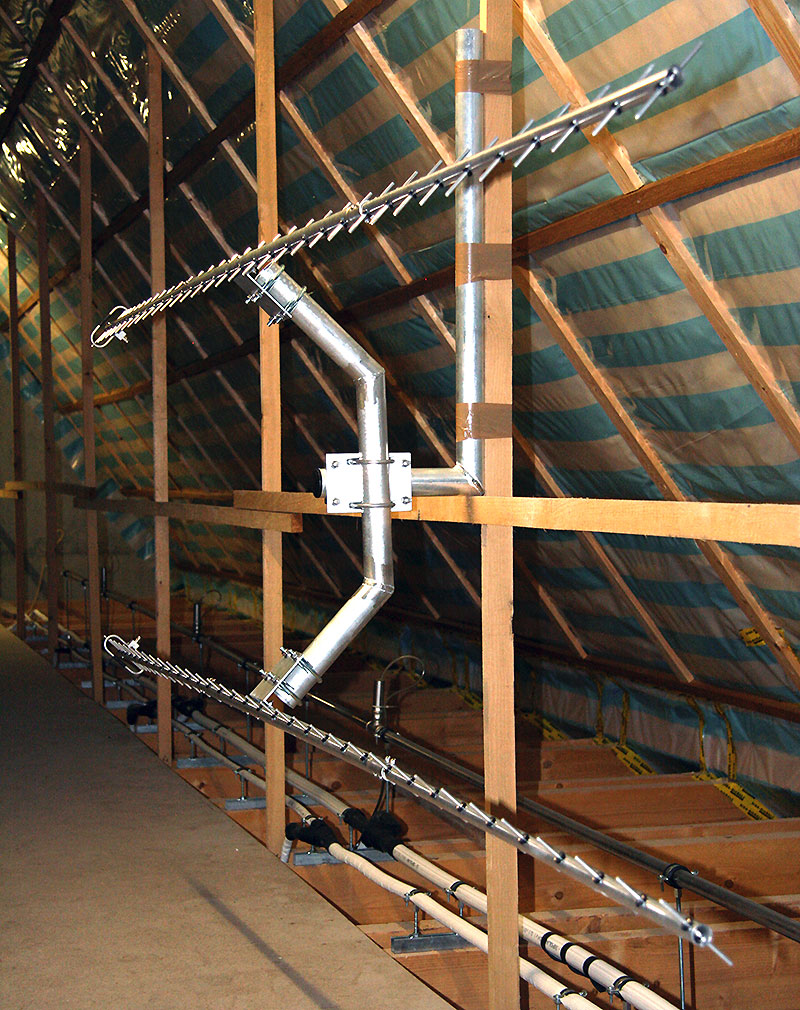
\includegraphics[width=\textwidth]{images/antenne3}
	\end{minipage}
	\caption[Antennen]{436CP42UG 70-cm, WX220 2-m und 23CM35 23-cm, Quelle: \cite{dk0te}}
	\label{fig: antennen}
\end{figure}
\newpar
Dazu gehört ein Mast sowie Vorverstärker und Polarisationsschalter. Die Antennen für das 23- und 70-cm-Band kommen von der Firma M$^2$ und die 
Antenne für das 2-m-Band von der Firma WIMO. Yagiantennen bestehen aus einem Faltdipol, einem Reflektor und mehreren Direktoren. Aus der Vorlesung 
Hochfrequenztechnik \cite{hfscript} ist bekannt, dass ein Reflektor ca. 5 $\%$ länger als $\frac{\lambda}{2}$ ist, somit oberhalb seiner 
Resonanzfrequenz betrieben wird und daher induktiv wirkt.  Anders ist es beim Direktor. Dieser wird von Direktor zu Direktor um ca. 5 $\%$ kürzer und 
wird im unteren Resonanzfrequenzbereich betrieben. Der Reflektor erhöht den Antennengewinn durch Reflexion der einfallenden Wellen auf dem Dipol. Die 
Direktoren beeinflussen die Abstrahlcharakteristik der Antenne, da die keulenförmige Ausprägung stärker wird. Bei der linken Kreuzyagi-Antenne sieht 
man in der Grafik den Reflektor und dahinter, den Faltdipol. Darauf folgen die Direktoren. Folgende Antennengewinne werden von den Antennen 
bereitgestellt: 436CP42UG (70-cm): 18.90 dBic, 23CM35 (23-cm): 20.94 dBi und WX220 (2-m): 35.00 dBi.

\subsection{Rotoren}
\label{chap:rotoren}
Um die Richtantennen steuern zu können werden Rotoren sowie dessen Steuergeräte von der Bodenstation zur Verfügung gestellt.
\begin{figure}[h]
	\centering
	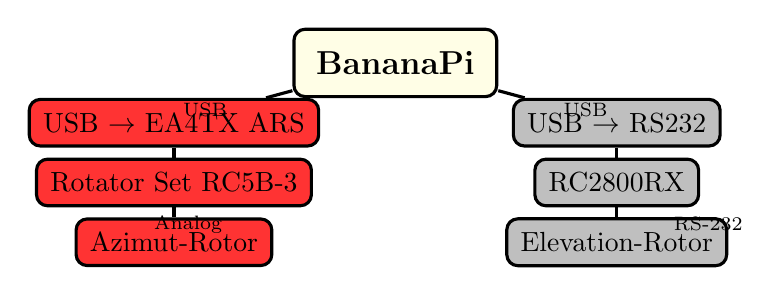
\begin{tikzpicture}[every node/.style = {shape=rectangle, rounded corners, draw, align=center, scale=1}, line width=0.4mm, level 
distance=1.8\baselineskip, level 1/.style = {sibling distance=16em}, level 2/.style = {sibling distance=8em}]
	\tikzstyle{top} = [fill=yellow!10, inner sep=8pt, font=\bfseries\large]
	\tikzstyle{az} = [fill=red!80, inner sep=5pt]
	\tikzstyle{el} = [fill=gray!50, inner sep=5pt]
	\tikzstyle{label} = [draw=none, font=\scriptsize, right]
	\node[top]{BananaPi}
	child { node[az]{USB $\rightarrow$ EA4TX ARS} 
		child { node[az]{Rotator Set RC5B-3} 
		  child { node[az]{Azimut-Rotor} } } }
	child { node[el]{USB $\rightarrow$ RS232}
		child { node[el]{RC2800RX}
		  child { node[el]{Elevation-Rotor} } } };
	\node[label] at (2,-0.6) {USB};
	\node[label,left] at (-2,-0.6) {USB};
	\node[label] at (-3.2,-2.05) {Analog};
	\node[label] at (3.4,-2.05) {RS-232};
% 	\node[label] at (-3.2,-3.5) {};
% 	\node[label] at (3.4,-3.5) {};
\end{tikzpicture} 

	\caption{Rotorsteuerung}
	\label{fig:azel}
\end{figure}\\
In der Abbildung \ref{fig:azel} stellt der BananaPi, ein Einplatinencomputer, die Rotorsteuerung als Einheit in dem DHBW Netzwerk bereit. Über die 
ARSVCOM Schnittstelle kann auf ihn zugegriffen werden. Die Bodenstation verfügt über zwei unterschiedliche Steuergeräte für den Elevationsrotor und 
den Azimutrotor. Dieser BananaPi emuliert zwei einheitliche Steuergeräte und setzt die Kommandos des ARS Protokolls um. Über USB sind die 
Steuergeräte für den Azimut- und Eleavtions-Rotor an den BananaPi angeschlossen. Das Steuergerät RC2800PXEL für den 
Elevationsrotor von der Firma M$^2$ arbeitet mit der seriellen Schnittstelle RS-232. Daher wird ein USB $\rightarrow$ RS232 Adapter benötigt. Das 
analoge Steuergerät RC5B-3-P von Create für den Azimutrotor benötigt einen Umsetzer von dem digitalen in den analogen Bereich. Dies geschieht über 
das Antennen-Rotor System ARS-USB von EA4TX. 
% \begin{figure}[h]
% 	\centering
% 	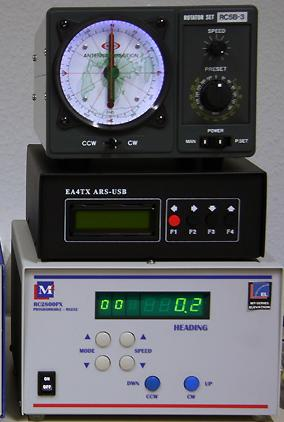
\includegraphics[width=0.225\textwidth]{images/sat-rotor-steuerungen}
% 	\caption{Steuergeräte für die Rotorsteuerung}
% 	\label{fig:rot}
% \end{figure}
% \newpar
% In der Grafik \ref{fig:rot} sind die Steuergeräte zu sehen.
\clearpage
\subsection{Funkgerät ICOM IC-9100}
\label{chap:funkgerät}
\begin{figure}[h]
	\centering
	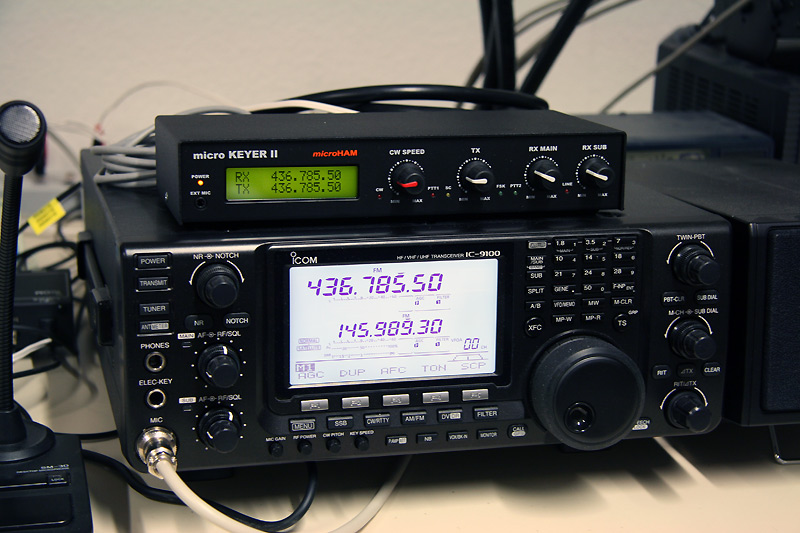
\includegraphics[width=0.6\textwidth]{images/radio}
	\caption[Funkgerät ICOM IC-9100]{Funkgerät ICOM IC-9100, Quelle: \cite{dk0te}}
	\label{fig:radio}
\end{figure}
Die letzte zentrale Komponente der Bodenstation ist das Funkgerät und ermöglicht den Funkbetrieb. Das IC-9100 Funkgerät der Firma ICOM ist ein 
Multiband Transceiver mit Doppelempfangsmöglichkeit, da der IC-9100 über drei unabhängige Empfängerschaltungen verfügt.Die Sendebandbreite ist durch 
wählbare Hochpass- und Tiefpassfrequenz einstellbar und das Funkgerät verfügt über eine Sendeleistung von 100 Watt. Eine für die Bodenstation 
wichtige Funktion ist der Funkbetrieb über Amateurfunksatelliten. Im einstellbaren Satellitenbetrieb synchronisiert der IC-9100 die Sende-  und 
Empfangsfrequenz und stimmt beide mit der gleichen Abstimmschrittweite ab. Das Funkgerät kann in den Satelliten Modi B (435 MHz Uplink, 145 MHz 
Downlink) und J ( 145 MHz Uplink, 435 MHz Downlink) betrieben werden. Die Kommunikation über den PC mit dem Funkgerät erfolgt über die Software 
Netcom.  Das Netcom-Modul ist mit dem ICOM IC-V Bus verbunden und bietet neben einer USB-Schnittstelle mit emulierter 
Soundkarte auch eine Netzwerkschnittstelle über die man mit dem Netcom Manager (der wiederum eine virtuelle serielle Schnittstelle zur Verfügung 
stellt) mit dem Funkgerät kommunizieren kann. Das IC-9100 kann die wichtigsten Amateurfunkbänder, von Kurzwelle bis \ac{UHF}, 
erfassen. 



% 	\item Funkgerät Icom IC-9100
% 	\begin{itemize}
% 		\item Netcom (2x Seriell zu Ethernet)
% 		\item Netcom Manager Software
% 		\item Hardware für Sprechfunk ?!
% 	\end{itemize}
% \end{itemize}


